\section{Validation on Simulated Data} %Toy Example
\label{sec:experiment_toy}

\begin{figure}%
    \centering
    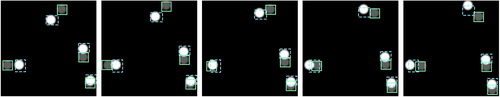
\includegraphics[width=0.99\textwidth]{figures/MOHART/sot_protons}
    \caption{\textsc{hart} single object tracking applied four times in parallel. Dashed lines indicate spatial attention, solid lines are predicted bounding boxes at time step $T+3$, faded circles show the ground truth location at $T+3$. The repulsive force between each object pair scales with distance as $1/r$. There is no information exchange between the trackers and each tracker evidently only `attends' to its own object. The fact that the future location is predicted accurately (i.e., much better than linear extrapolation) indicates that \textsc{hart} is able to capture complex motion patterns essentially allowing to draw conclusions about the force field. Shown are consecutive time steps from left to right.
    }
    \label{fig:toy1}
\end{figure} 
\begin{figure}%
    \centering
    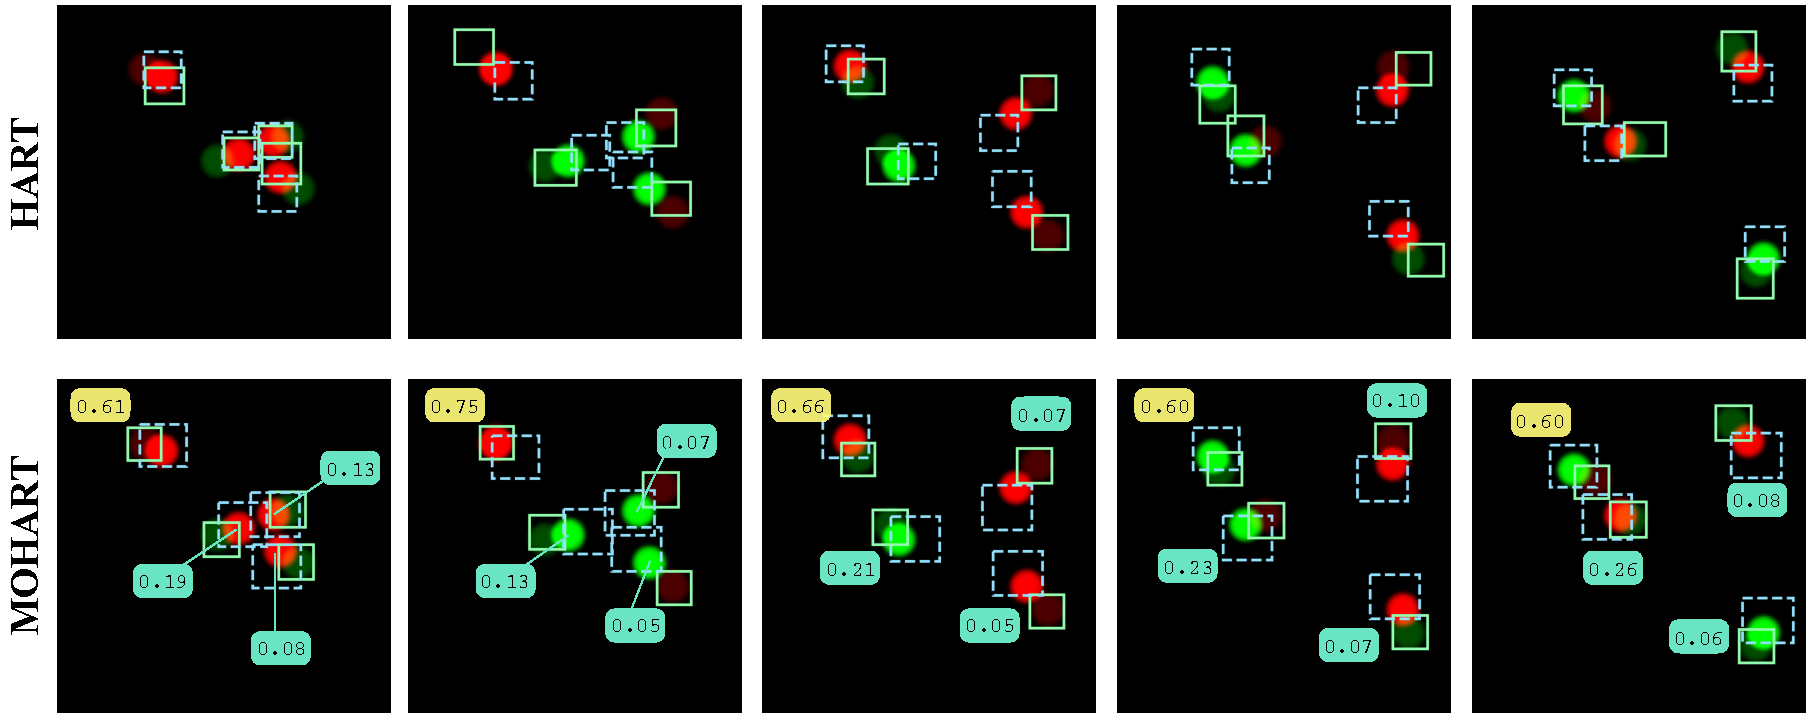
\includegraphics[width=0.99\textwidth]{figures/MOHART/mot_proel}
    \caption{\textsc{hart} (top, $46\%$ IoU) vs. \textsc{mohart} (bottom, $76\%$ IoU). Dashed lines show spatial attention, solid lines show predicted bounding boxes, faded circles indicate future ground truth locations. Circles of the same colour repel each other, circles of different colours attract each other. The colour coded identities are randomly assigned in each time step rendering information exchange between trackers (i.e. relational reasoning) necessary. The numbers in the bottom row indicate the self-attention weights from the perspective of the top left tracker (yellow number box).
    }
    \label{fig:toy2}
\end{figure}


To test the efficacy of the proposed algorithm, we conduct experiments on a toy domain. First, we show that \textsc{hart} as an end-to-end single-object tracker is able to capture complex motion patterns and leverage these to make accurate predictions. Second, we create a scenario which is not solvable for a single object tracker as it requires knowledge about the state of the other objects and relational reasoning. We show that \textsc{mohart}, using self-attention for relational reasoning, is able to capture these interactions with high accuracy and compare it to other possible implementations of \textsc{mohart} (e.g., using max-pooling instead of self-attention). In order to accurately investigate the model's understanding of motion patterns and interactions between objects, in contrast to traditional tracking, the model is not trained to predict the current location of the object, but its location in a future time step. The domain we create for this purpose is a two dimensional squared box. It contains circular objects with approximated elastic collisions (energy and momentum conservation) between objects and with walls (see \Cref{fig:toy1,fig:toy2}).

In the first scenario (\Cref{fig:toy1}), four circles each exert repulsive forces on each other, where the force scales with $1/r$, $r$ being their distance. \textsc{hart} is applied four times in parallel and is trained to predict the location of each circle three time steps into the future. The different forces from different objects lead to a non-trivial force field at each time step. Predicting the future location just using the previous motion of one object (\Cref{fig:toy1} shows that each spatial attention box covers only the current object) accurately is therefore challenging. Surprisingly, the single object tracker solves this task with an average of $95\%$ IoU over sequences of 15 time steps. This shows the efficacy of end-to-end tracking to capture complex motion patterns and use them to predict future locations. This, of course, could also be used to generate robust bounding boxes for a tracking task.

The second scenario (\Cref{fig:toy2}) is constructed to be impossible to solve without exchanging information between objects. This is achieved by introducing two colour-coded identities. Agents of the same identity repel each other, agents of different identities attract each other. Crucially, each agent is randomly assigned its identity in each time step. Hence, the algorithm can no longer infer the forces exerted on one object without knowledge of the state of the other objects in the current time step. The forces in this scenario scale with $1/\sqrt{r}$ and the algorithm was trained to predict one time step into the future. \textsc{hart} is indeed unable to predict the future location of the objects accurately (\Cref{fig:toy2} - top). The achieved average IoU is $47\%$, which is only slightly higher than predicting the objects to have the same position in the next time step as in the current one ($34\%$). A possible interpretation of the qualitative results (green boxes in \Cref{fig:toy2} - top) is that the model uses the momentum of each object to extrapolate into the future. This sometimes works well (bottom right object in frame 31) and sometimes not (top right object in frame 30). Using the relational reasoning module (\Cref{fig:toy2} - bottom), the model is now able to make meaningful predictions ($76\%$ IoU). Interestingly, in each frame, the attention scores have a strong correlation with the interaction strength (which directly scales with distance). Despite this not being necessary for the relational reasoning module, this is an interesting side-product as it did not receive any direct supervision.

\begin{figure}
    \centering
    \begin{subfigure}[c]{0.49\linewidth}
        \centering
        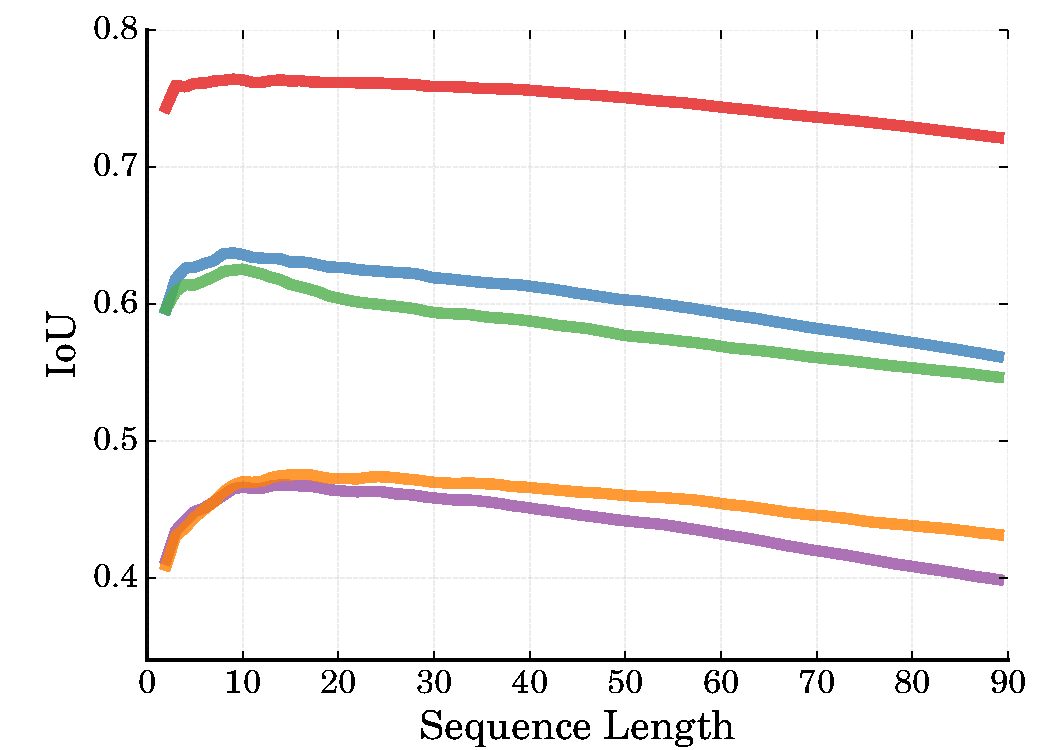
\includegraphics[width=\linewidth]{figures/MOHART/toy_iou_over_timesteps}
    \end{subfigure}
    \begin{subfigure}[c]{0.49\linewidth}
        \centering
        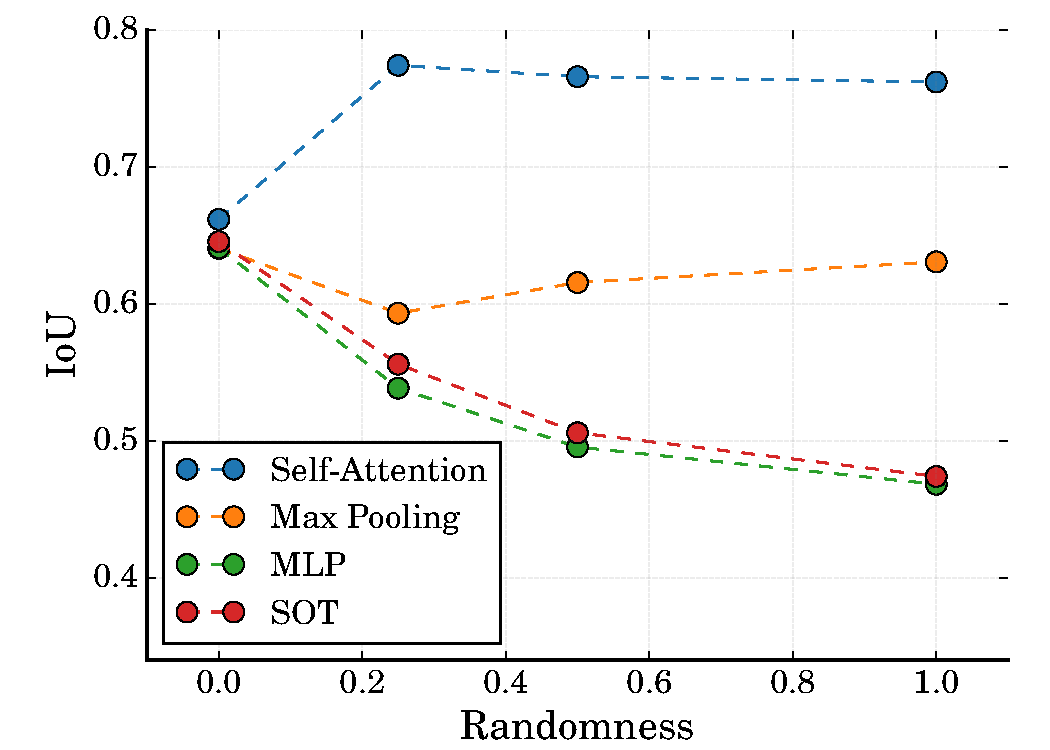
\includegraphics[width=\linewidth]{figures/MOHART/dial}
    \end{subfigure}
    \caption{
        Left: average IoU over sequence length for different implementations of relational reasoning on the toy domain shown in \cref{fig:toy2} ($\text{randomness} = 1.0$). Right: performance depending on how often agents are re-assigned identities randomly (sequence length 15). The higher the randomness, the less static the force field is and the more vital relational reasoning is. 
    }
    \label{fig:toy_quant}
\end{figure}

\Cref{fig:toy_quant} (left) shows a quantitative comparison of augmenting \textsc{hart} with different relational reasoning modules when identities are re-assigned in every timestep ($\text{randomness} = 1.0$). Exchanging information between trackers of different objects in the latent space with an MLP leads to slightly worse performance than the SOT baseline, while simple max-pooling performs significantly better ($\Delta \text{IoU} \sim 17\%$). This can be explained through the permutation invariance of the problem: the list of latent representation of the different objects has no meaningful order and the output of the model should therefore be invariant to the ordering of the objects. The MLP is in itself not permutation invariant and therefore prone to overfit to the (meaningless) order of the objects in the training data. Max-pooling, however, is permutation invariant and can in theory, despite its simplicity, be used to approximate any permutation invariant function - given a sufficiently large latent space \cite{Zaheer2017,Wagstaff2019}. Max-pooling is often used to exchange information between different tracklets, e.g., in the trajectory prediction domain \cite{Alahi2016social,Gupta2019social}. However, self-attention, allowing for learned querying and encoding of information, solves the relational reasoning task significantly more accurately. In \Cref{fig:toy_quant} (right), the frequency with which object identities are reassigned randomly is varied. The results show that, in a deterministic environment, tracking does not necessarily profit from relational reasoning - even in the presence of long-range interactions. The less random, the more static the force field is and a static force field can be inferred from a small number of observations (see \Cref{fig:toy1}). This does of course not mean that all stochastic environments profit from relational reasoning. What these experiments indicate is that tracking can not be expected to profit from relational reasoning by default in any environment, but instead in environments which feature (potentially non-deterministic) dynamics and predictable interactions.